\section{Introduction}

% TODO: use or not?
% \begin{frame}{StroemungsRaum consortium}
% 	% \hspace*{-2cm}
% 	% \vspace*{-1cm}
% 	\begin{figure}
% 		\centering
% 		\scalebox{0.8}{ % Adjust scale if needed
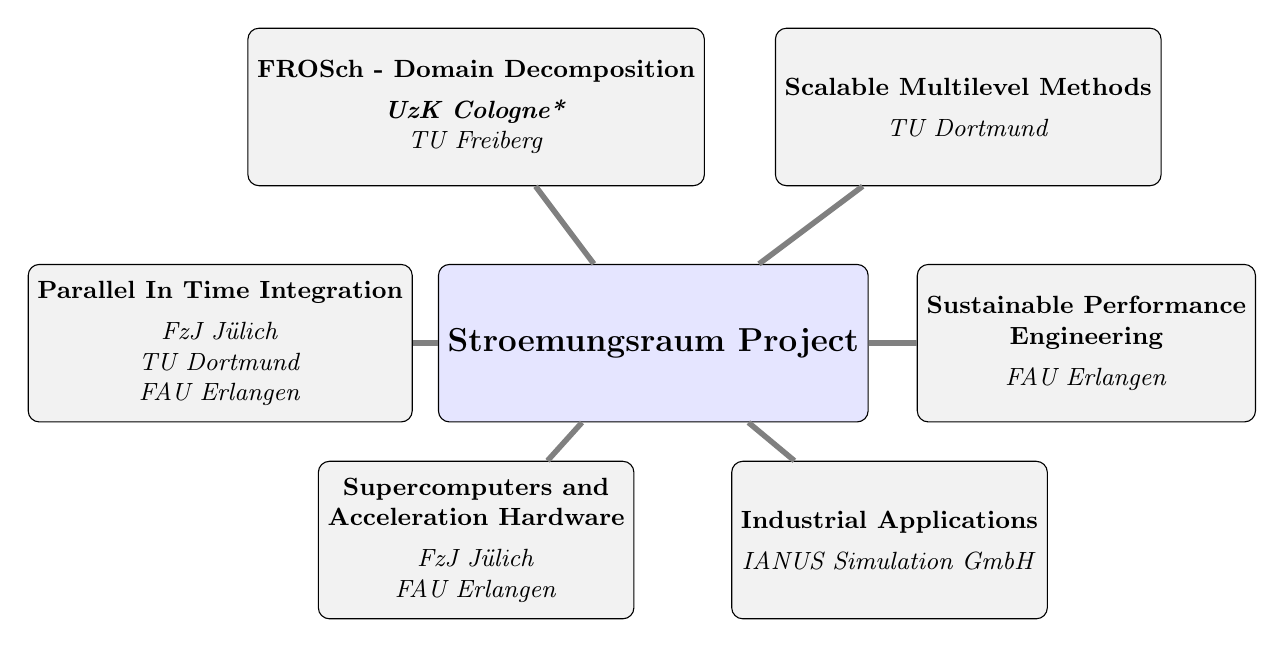
\begin{tikzpicture}[
  % Removed "mindmap" as it applies specific styling that's hard to override
  every node/.style={
    rectangle,
    rounded corners,
    minimum width=2cm,
    minimum height=2cm,
    align=center,
    font=\small,
    text=black,
    draw=black,
    fill=gray!10
  },
  root concept/.style={
    fill=blue!10,
    font=\bfseries\large,
    text=black,
    minimum width=3cm
  },
  % Custom edge style
  conn/.style={
    draw=black!50,
    line width=2pt,
    solid
  },
]
\node[root concept] (root) {Stroemungsraum Project};

% Create child nodes with explicit positioning and manual edges
\node[xshift=5.5cm, yshift=0cm] (n1) {\bf{Sustainable Performance}\\\bf{Engineering}\\[1ex] \textit{FAU Erlangen}};
\node[xshift=4cm, yshift=3cm] (n2) {\bf{Scalable Multilevel Methods}\\[1ex] \textit{TU Dortmund}};
\node[xshift=-2.25cm, yshift=3cm] (n3) {\bf{FROSch - Domain Decomposition}\\[1ex]\textit{\textbf{UzK Cologne*}}\\ \textit{TU Freiberg}};
    \node[xshift=-5.5cm, yshift=0cm] (n4) {\bf{Parallel In Time Integration}\\[1ex] \textit{FzJ Jülich}\\ \textit{TU Dortmund}\\ \textit{FAU Erlangen}};
\node[xshift=-2.25cm, yshift=-2.5cm] (n5) {\bf{Supercomputers and}\\\bf{Acceleration Hardware}\\[1ex] \textit{FzJ Jülich}\\\textit{FAU Erlangen}};
    \node[xshift=3cm, yshift=-2.5cm] (n6) {\bf{Industrial Applications}\\[1ex] \textit{IANUS Simulation GmbH}};
%
% % Draw thin connections
\draw[conn] (root) -- (n1);
\draw[conn] (root) -- (n2);
\draw[conn] (root) -- (n3);
\draw[conn] (root) -- (n4);
\draw[conn] (root) -- (n5);
\draw[conn] (root) -- (n6);
\end{tikzpicture}
}

% 	\end{figure}
% \end{frame}

\begin{frame}{Some References on Nonlinear Domain Decomposition Methods}
	\tiny
	\textbf{Nonlinear FETI-DP and Nonlinear BDDC:}\\
	Klawonn, Lanser, Rheinbach (2012, 2013, 2014, 2015, 2016, 2018), Klawonn, Lanser, Rheinbach, Uran (2017, 2018), Klawonn Lanser, Uran (2021, 2023), \dots\\~\\

	\textbf{Nonlinear Elimination:}\\
	Hwang, Lin, Cai (2010); Cai, Li (2011); Wang, Su, Cai (2015); Hwang, Su, Cai (2016); Gong, Cai (2018); Luo, Shiu, Chen, Cai (2019); Gong, Cai (2019); Liu, Hwang, Luo, Cai, Keyes (2022), \dots\\~\\

	\textbf{ASPIN:}\\
	Cai, Keyes 2002; Cai, Keyes, Marcinkowski 2002; Hwang, Cai 2005, 2007; Groß, Krause (2010, 2013), \dots\\~\\

	\textbf{MSPIN and Field-split methods:}\\
	Keyes, Liu, (2015, 2016,2021); Liu, Wei, Keyes (2017); Kopanicáková, Kothari, Krause (2023), \dots\\~\\

	\textbf{RASPEN:}\\
	Dolean, Gander, Kherijii, Kwok, Masson (2016)\\~\\

    \hspace*{-2.7mm}
    \noindent\fcolorbox{red}{white}{
        \begin{minipage}{0.4\textwidth}
            \textbf{Nonlinear 2-Level Schwarz:}\\
			Heinlein, Lanser (2020); Heinlein, Klawonn, Lanser (2022)
		\end{minipage}}\\~\\

	\textbf{Nonlinear Neumann-Neumann:}\\ Bordeu, Boucard, Gosselet 2009\\~\\

	\textbf{Nonlinear FETI-1:}\\
	Pebrel, Rey, Gosselet 2008; Negrello, Gosselet, Rey (2021)\\~\\

	\textbf{Other DD work reversing linearization and decomposition:}\\
	Ganis, Juntunen, Pencheva, Wheeler, Yotov 2014; Ganis, Kumar, Pencheva, Wheeler, Yotov 2014
\end{frame}

\begin{frame}{Two-level nonlinear Schwarz}%: Nonlinearly preconditioned inexact Newton algorithms}}
	\begin{tikzpicture}[transform shape]
    % Define coordinates for the main elements
    \coordinate (leftImg) at (0,0);
    \coordinate (topImg) at (5,2.5);
    \coordinate (bottomImg) at (5,-2.5);
    \coordinate (rightEq) at (10,1.0);
    
    % Place the placeholder images (blue rectangles with numerical solution)
    \node[inner sep=0] (leftRectangle) at (leftImg) 
        {\includegraphics[width=5cm]{images/global-solution.png}};
    \node[inner sep=0] (topRectangle) at (topImg) 
        {\includegraphics[width=5cm]{images/coarse-solution.png}};
     \node[inner sep=0] (bottomRectangle) at (bottomImg) 
        {\includegraphics[width=5cm]{images/local-solutions.png}};
    
    \node[yshift=5mm, xshift=2mm, text width = 35mm, font=\small] at (leftRectangle.north) {Discretized nonlinear problem};
    \node[yshift=-2mm, font=\small] at (leftRectangle.south) {$F(u) = 0$};

    \node[yshift=-2mm, font=\small] at (bottomRectangle.south) {$R_i F\left(u - P_i T_i(u)\right) = 0$};
    
    \node [yshift=-2mm, font=\small] at (topRectangle.south){$R_0 F\left(u - P_0 T_0(u)\right) = 0$};
    
    \node[align=left, text width = 4.5cm, font=\small] at (9.6,-1.3){Solve with Newton's method for nonlinear corrections $T_i(u) \text{ for } i = 1,2,\dots,N$};
    
    \node[draw, rectangle, minimum width=4cm, minimum height=1cm, font=\small] (boxedEq) at (rightEq) {$\mathcal{F}(u) = \sum_{i=0}^{N} P_i T_i(u) = 0$};
    
    % Arrows
    \draw[-{Stealth[length=3mm, width=2mm]}] ($(leftRectangle.north east) + (-0.5, -0.5)$) -- ($(topRectangle.south west) + (0.3, 0.3)$);
    \draw[-{Stealth[length=3mm, width=2mm]}] ($(leftRectangle.south east) + (-0.7, 0.4)$) -- ($(bottomRectangle.north west) + (0.8, -0.2)$);
    \draw[-{Stealth[length=3mm, width=2mm]}] ($(topRectangle.south east)+ (-0.3, 0.7)$) -- ($(boxedEq.north west)+ (-0.1, 0.1)$);
    \draw[-{Stealth[length=3mm, width=2mm]}] ($(bottomRectangle.north east)+ (-0.8, -0.1)$) -- ($(boxedEq.south west)+ (-0.1, -0.1)$);
\end{tikzpicture}

\end{frame}

\begin{frame}{Software ecosystem}
	\begin{tikzpicture}[node distance = 1cm, auto]

	\node [whtblock,text depth=14mm] (FEDDLIB) {
		{\footnotesize \textbf{FEDDLib}\textsuperscript{a}} \\[0.3em] \tiny \textbf{F}inite \textbf{E}lement and \textbf{D}omain \textbf{D}ecomposition \textbf{Lib}rary
		\begin{itemize}
			\item{Parallel finite element assembly}
			\item{Specific problem definition}
			\item{Mesh handling routines}
			      % \item \textcolor{orange}{Update two-level nonlinear Schwarz solver for elasticity and Navier-Stokes}
			      % \item \textcolor{orange}{Test with various coarse spaces}
		\end{itemize}
		% \hspace*{-25mm}\scalebox{.7}{By University of Cologne, TU Delft, TU Freiberg}
	};

	\node [whtblock, right=of FEDDLIB,node distance=7cm, rectangle split part fill={orange!20,blue!5},] (FeatFlow) {
		{ \footnotesize\textbf{FEATFLOW}\textsuperscript{b}}\\[0.3em] \tiny Finite element based solution of incompressible\\Navier-Stokes in 2D and 3D
		\vspace{2pt}
		\begin{itemize}
			%\setlength{\itemsep}{0pt}
			\item \textcolor{red}{Interface with \texttt{FROSch}}
			\item \textcolor{red}{Test (non-Newtonian, high Reynolds, exascale)}
		\end{itemize}};

	%===============================================    
	\node [whtblock, below=of FEDDLIB, text depth=18mm, node distance=3.5cm,] (Trilinos) {
		{\footnotesize \textbf{Trilinos}\textsuperscript{c}}
		\begingroup
		\addtolength{\leftmargini}{0.5cm}
		\vspace{1pt}
		\tiny
		\begin{itemize}
			%\setlength{\itemsep}{0pt}
			\item Data services: Vectors, matrices, graphs and related operations
			\item Linear and Eigenproblem solvers
			\item Nonlinear solvers and analysis tools
		\end{itemize}
		\endgroup
	};

	\node[inner sep=0pt] (trilinos_logo) at ([xshift=6mm, yshift=0mm] Trilinos.west){\includegraphics[width=.125\textwidth, angle=90,origin=c]{images/logo/Trilinos_logo_new.png}};

	\node [whtblock, text depth=18mm, right=of Trilinos,node distance=7cm,rectangle split part fill={orange!20,blue!5},] (Frosch) {
		{\footnotesize \textbf{FROSch}\textsuperscript{d}} \\[0.4em]  \hspace{6em}\tiny\textbf{F}ast and \textbf{R}obust \textbf{O}verlapping \textbf{S}chwarz
		\vspace*{0.5em}
		\begingroup
		\addtolength{\leftmargini}{4em}
		\begin{itemize}
			\item \textcolor{red}{Implement two-level nonlinear Schwarz solver}
			\item \textcolor{red}{Test with various coarse spaces on various model problems}
		\end{itemize}
		\endgroup
	};

	\node[inner sep=0pt] (trilinos_logo) at ([xshift=7.5mm, yshift=0mm] Frosch.west){\includegraphics[width=.1\textwidth]{images/logo/FROSch_logo.png}};

	%%%%%%%%%%%%%%%%%%%%%%%%%%%%%%%%
	%   CONTAINERS -- BACKGROUND LIGHT-DASHED BLOCKS
	%%%%%%%%%%%%%%%%%%%%%%%%%%%%%%%%
	\begin{scope}[on background layer]

		\coordinate (aux2) at ([yshift=0mm]Trilinos.north);
		\node[container2, fit=(aux2) (Trilinos) (Frosch)] (Trilinos_blue) {};

		\coordinate (aux3) at ([yshift=0mm] FeatFlow.north);
		\node[container3, fit=(aux3) (FeatFlow)] (FeatFlow_Green) {};

		\coordinate (aux1) at ([yshift=0mm]FEDDLIB.north);
		\node [container,fit=(aux1) (FEDDLIB)] (FEDDLIB_ORANGE) {};
		\node at ([yshift=0.7mm]Trilinos_blue.north) [fill=gray!10,draw,minimum width=8em,minimum height=1em] (FEDTRI-label) {\footnotesize\textbf{Interface}};

	\end{scope}
	%************************************************************
	%************************************************************
	%  Draw edges
	%************************************************************
	%************************************************************
	% \path [line,thick] (FEDDLIB) -- (FEDTRI-label);
	% \path [line,thick] (Trilinos) -- (Frosch);
	% \path [line,thick] (FEDTRI-label) -- (Trilinos);
	% \path [line,red,thick] (FeatFlow) -- (FEDTRI-label);

\end{tikzpicture}
\tiny\\~\\

a: University of Cologne, TU Delft, TU Freiberg (https://github.com/FEDDLib/FEDDLib.git)\\
b: TU Dortmund (https://wwwold.mathematik.tu-dortmund.de/~featflow/en/software.html)\\
c: Sandia National Laboratories (https://trilinos.github.io)\\
d: University of Cologne, TU Delft, TU Freiberg (https://shylu-frosch.github.io)\\

\end{frame}


